\section{Background}
\subsection{Motivation}
Data is a crucial resource in all economic and social activities of our society, with an estimated 16 zettabytes of useful data (16 Trillion GB) \cite{a} to be accumulated by 2020. Data sources are omnipresent in our lives, including streams from financial markets, video monitoring systems, social media streams and web activity logs. Exploiting this data to increase competitiveness in an increasingly data-driven socioeconomic model will boost innovation and drive cutting-edge technologies, which is key to economic growth. The demosEUROPA \cite{b} estimated that ‘Overall, by 2020, big \& open data can improve the European GDP by 1.9\%, an equivalent of one full year of economic growth in the EU’, while the International Data Corporation (IDC) \cite{c} shows that large companies and SMEs are accelerating their adoption of Big Data as they recognise the market value proposition and need to step forward into the data-driven economy.

Despite the great demand for Big Data, the development and deployment of Data Intensive Applications (DIAs) requires significant expertise and remains relatively inaccessible to new and less experienced programmers. The configuration of underlying technologies such as Hadoop, Spark, and Storm, has a significant impact on the performance of DIAs up to orders of magnitude \cite{bo4co}. This requires expert administrators with clear understanding of the technologies used, in order to test and tune the systems using a mix of trial-and- error and heuristic methods. Even with experienced administrators, manual configuration is virtually impossible due to the number of configuration parameters and possibly nonlinear interaction between them.

The Big Data Auto-Tuning tool is a solution to finding optimum configuration for DIAs, helping developers with little or no knowledge of the underlying big data technologies automatically improving their application’s performance. The following sections further detail the current state of tools, which consists of separate parts including the BO4CO tool, test runners and monitoring tool. The main aim of this project is to provide an environment that:
\begin{itemize}
\item Fully integrates with DICE project development environment as an Eclipse IDE plugin
\item Facilitates continuous integration by providing automated deployment and performance testing of big data applications
\item Automatically detects optimal configuration to enhance big data application performance without requiring developer knowledge of underlying system 
\end{itemize}
\newpage

\subsection{DICE Project}
DICE is a project on quality-driven development of Big Data applications.\cite{dice} It researches methodology and tool chain to allow high quality, high performance Big Data applications to be developed with less experience and less domain-specific expertise required. The project covers quality assessment, architecture enhancement, continuous testing and agile delivery based on the DevOps paradigm. 

The DICE framework is structured as in Figure \ref{fig:dice}, and divided into four main components \cite{dicetools}:
\begin{itemize}
\item DICE IDE: for coding, design and prototyping
\item Quality Analysis Tools: by simulation, verification and optimization
\item Feedback and Iterative Enhancement Tools: a resource, performance and anomaly monitoring platform tailored for Big Data technologies
\item Continuous Delivery and Testing Tools: with continuous integration, delivery on clouds and optimal application configuration
\end{itemize}
\begin{figure}[h]
\centering
\caption{DICE framework. \cite{dicetools}}
\label{fig:dice}
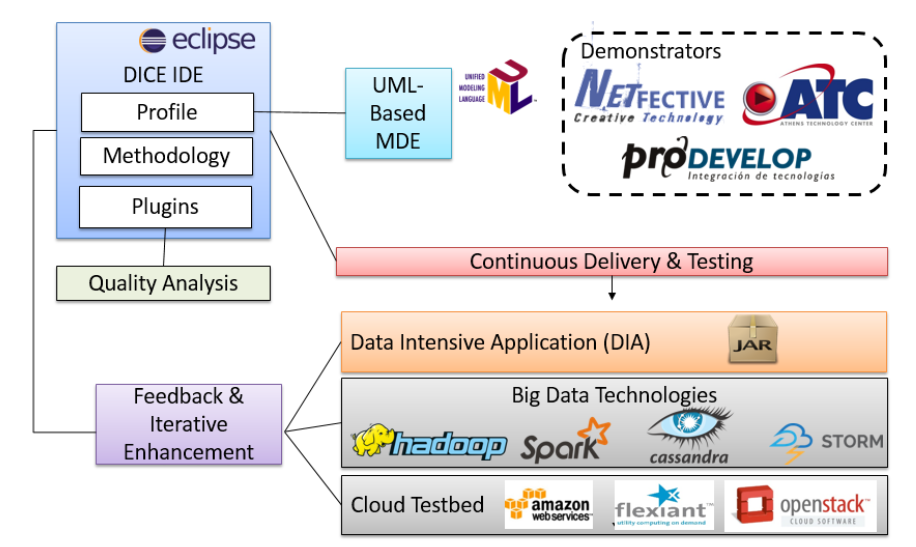
\includegraphics[width=0.9\textwidth]{images/dice.png}
\end{figure}

\newpage
\subsubsection{DICE IDE}
The DICE IDE is an integrated development environment built on the Eclipse IDE. It provides MDE functionality to model Big Data applications and the Big Data technologies behind. It is the front-end user interface for integration of all DICE tool chain components.
\subsubsection{Quality Analysis Tools}
The Quality Analysis Tools assess requirements and parameters specified in UML design for performance, reliability and safety. The Transformation Tools produce formal models, such as stochastic Petri nets, for validation and simulation in the Simulation Tools. The safety properties are checked using Verification Tools, then the Optimization Tools evaluate optimal deployment configuration using Petri net models. 
\subsubsection{Feedback and Iterative Enhancement Tools}
The monitoring platform provides feedback by analysing traces and logs stored during execution of application on Big Data framework. Anomaly Trace Tools apply machine learning algorithms to enable the detection of quality incidents and anti-patterns based on classification, statistical analysis and trace analysis. Enhancement tools correlate monitor data to the application's design models, and guides quality improvement.
\subsubsection{Continuous Delivery and Testing tools}
The Continuous Integration and Deployment tools set up the testbed and deploy the application to pre-production environment, where quantitative performance and reliability feedback on test input feeds is assessed as part of a DevOps work flow. The integration of automated deployment and testing tools internally and with existing development tools such as Eclipse and Jenkins will be key objectives in this project, to provide a seamless work flow that improves development efficiency.

\newpage
\subsection{Configuration Optimization Tool}
Tuning the performance and reliability of Big Data applications is time consuming, as applications can involve several frameworks such as Apache Storm, Kafka, and Spark. The default parameters may not work optimally in different situations, and well-tuned systems can perform up to orders of magnitude better, making it crucial to find the optimal configuration \cite{bo4co}. Each framework has hundreds of configuration parameters that can present a few options or accept a range of values. There are $(num\_options)\wedge(num\_params)$ of possible configuration combinations, which easily reaches 1M possibilities when we choose to optimise 10 key parameters with 4 configuration options. A brute force approach that tested each possibility for 10 minutes of run time will take 19 years to find the optimal solution. The Configuration Optimization Tool has to find a good set of configuration parameters by experimentation within a limited time. A machine learning algorithm, BO4CO has been developed for this purpose, and is introduced in the next section. 
The Configuration Optimization Tool is structured as shown in Figure \ref{fig:cotool}, and has the following components:
\begin{itemize}
\item Configuration Optimizer (BO4CO)
\item Data Broker and performance repository
\item Experimental Suite: for running tests on Testbed and monitoring
\end{itemize}
\begin{figure}[h]
\centering
\caption{Configuration Optimization Tool. \cite{bo4cogit}}
\label{fig:cotool}
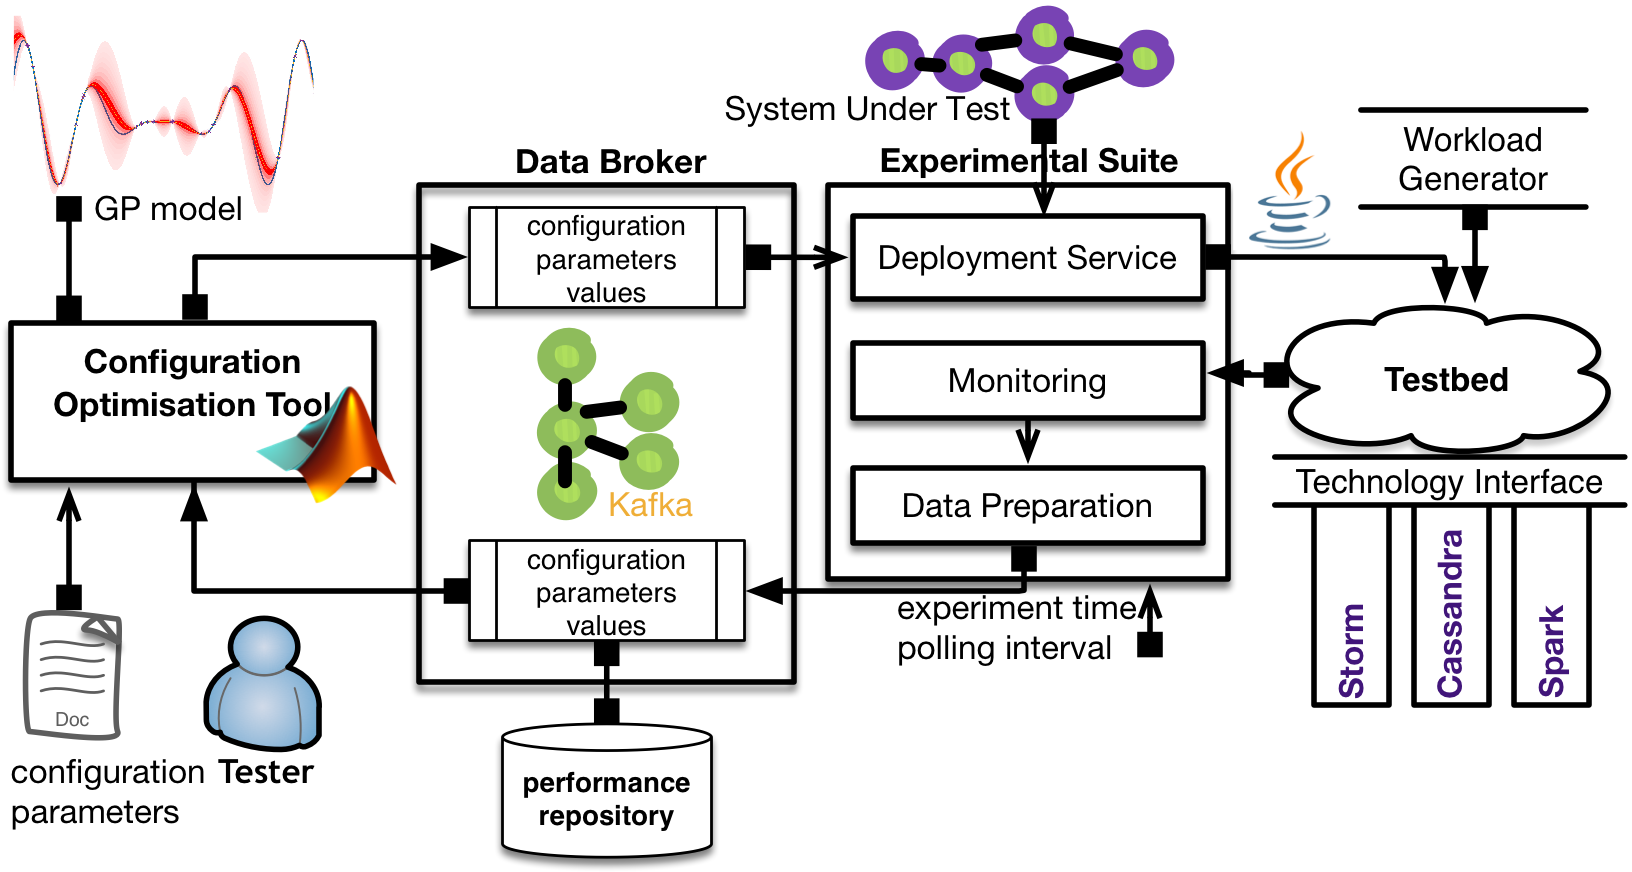
\includegraphics[width=0.9\textwidth]{images/cotool.png}
\end{figure}
The configuration optimization process: \cite{bo4co}
\begin{enumerate}
\item Initialisation: Tester inputs parameters and possible values to test
\item Iteration 0: Working iteratively, select next configuration to test based on existing known performance measures
\item Deployment: DICE deployment tool automatically deploys the configured system on a testbed
\item Monitoring: DICE monitoring tool measures and stores the performance of the configuration to be added to historical data
\item Next Iteration: Select next configuration to test by fitting historical data to a model, go to step 3
\item Result: Terminate after the limited time has been reached, reporting the optimal configuration.
\end{enumerate}

\subsubsection{BO4CO Algorithm}
BO4CO algorithm \cite{bo4co} is used by the Configuration Optimizer to automatically select the best configuration to test next. The Algorithm uses observed performance data to estimate the response surface of the Big Data system under testing, and uses the estimated data to search for points where there is a high probability the optimum configuration lies.
The goal is $$x* = argmin f(x)$$,
where $$X = Dom(X1) x ... x Dom(Xd)$$ is the configuration space
and $$yi = f(xi)$$ is the partially known response function

\begin{enumerate}
\item Initialisation: form initial Latin Hypercube Design
\item Initial Measurement: form initial estimate of underlying response function from measurement on initial design
\item Repeatedly accumulate data with $yi = f(xi) + \epsilon i$ where $\epsilon i$ is noise in measurement
\item Form GP $y = f(x) \sim GP(\mu(x), k(x,x')$, where $k(x,x')$ is the distance between $x$ and $x'$
\item Assuming $S1:t = {(x1:t, y1:t)|yi := f(xi)}$ is a collection of $t$ observations, the function values are drawn from 
\[ K = \left| \begin{array}{ccc}
k(x1,x1) & ... & k(x1,xt) \\
... & ... & ... \\
k(xt,x1) & ... & k(xt,xt) \end{array} \right|\] 
\item To fit a new GP model with observations accumulated so far:
\[ \left| \begin{array}{c}f1:t \\ ft+1 \end{array} \right| 
= \left| \begin{array}{cc}
K + \sigma ^2 I & k\\
k^T & k(xt+1,xt+1)\end{array} \right|,\]
where $k(x)^T = [k(x,x1) k(x,x2) ... k(x,xt)] $ and I is identity matrix
\item new GP model created:
$$PR(ft+1|S1:t, xt+1) = N(\mu t(xt+1), \sigma ^2(xt+1))$$,\\
where $$\mu t(x) = \mu (x) + k(x)^T(K + \sigma ^2 I)^-1 (y-\mu)$$\\
$$\sigma ^2 t(x) = k(x,x) + \sigma ^2 I - k(x)^T(K + \sigma ^2 I)^-1 k(x)$$
\item Select next configuration $xt+1$ to best tested: 
$$xt+1 = argmax \mu (x|M,S1:t)$$,\\
where the criteria $\mu$ uses Lower Confidence Bound, which trades-off between exploitation and exploration:
$$\mu LCB(x|M, S1:n) = argmin\mu t(x) - k \sigma t(x)$$

\end{enumerate}

\newpage
\subsection{Big Data Frameworks}
Big Data Frameworks or Big Data Platforms are the modern solution for storing and processing Big Data in the Petabyte and Exabyte scales. While tradition monolithic systems that scale vertically face physical limitations in their power, parallel distributed storage and processing systems that scale horizontally do not face the same limitation and can work in hundreds or thousands of nodes. These systems are controlled by new frameworks including Hadoop, Spark and Storm. This project focuses tailoring performance in Spark and Storm applications by recognising key configuration parameters and building specific profile templates through experimentation.

\subsubsection{Storm}
Storm shares the topology shape of a directed acyclic graph, similar to MapReduce. \cite{stormtut} The data transformation pipeline consists of spouts and bolts at the graph vertices, and named streams directing data across nodes on the edges. The difference in Storm and MapReduce is that Storm processes data in real time, making it easy to process unbounded streams. Storm topologies run indefinitely until killed, while MapReduce jobs will terminate and are processed in batches. 
The benefits that Storm offer is that it can process large volumes of high velocity data, up to one million 100 byte messages per second per node. It is scalable, fault tolerant and easy to operate. The guarantee that every message is processed makes it reliable. Use cases include real time analytics, online machine learning, continuous computation, distributed RPC and ETL.
\begin{figure}[h]
\centering
\caption{Storm architecture. \cite{diced1}}
\label{fig:storm}
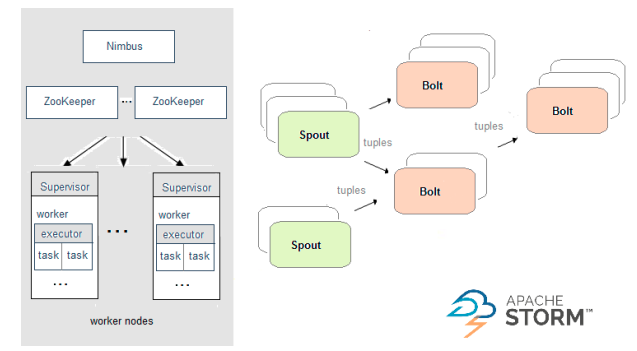
\includegraphics[width=0.9\textwidth]{images/storm.png}
\end{figure}

\newpage

\subsection{DevOps}
\subsubsection{Introduction to DevOps}
The term DevOps originated from "software DEVelopment" and "information technology OPerationS". 
DevOps is the combination of cultural philosophies, practices, and tools that aims to increase the speed, frequency and reliability in building, testing, and releasing software. 

Co-operation, collaboration and communication between software developers and Operations teams is the key difference championed in the DevOps paradigm, as opposed to the traditional separation of concerns. Before the rise of DevOps, developers in the "Dev" side were seen as the "creators", focused on innovating, implementing new features and improving the quality of the product. The "Ops" side involved system administration and maintenance, focused on "everything after the creation of the product", ensuring stability, availability and reliability. This rigid structuring of responsibilities could lead to friction as both roles affect the work of each other, and would instead benefit from the insights of the other in a more flexible system. 

The key ideas of DevOps are as shown in Figure \ref{fig:devops} \cite{d}:
\begin{itemize}
\item Software testing in an environment as close as possible to production environment, encouraging developers to consider operation issues including performance, availability and stability of application
\item Automation and remote deployment of application
\item Continuous monitoring of application throughout entire life-cycle
\item Feedback and collaboration between developers and operators to resolve issues and improve application considering the interest of both parties
\end{itemize}
\begin{figure}[h]
\centering
\caption{DevOps workflow.}
\label{fig:devops}
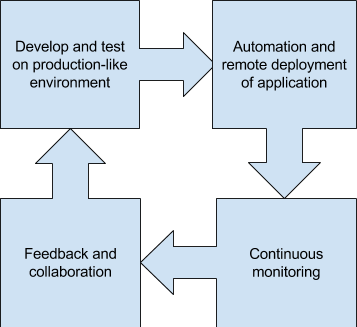
\includegraphics[width=0.5\textwidth]{images/devops.png}
\end{figure}
These practices aim to bridge the gap between developers and operators, encouraging them both to consider the perspective of the other, understand the basic of others domains, and share ideas, goals, issues, processes and tools \cite{e}. In this sense, DevOps is an extension to Agile practices that encourage quick iterations that deliver incremental improvements in the product. DevOps extends the idea across developers and operators, pushing both to quickly and frequently deliver product improvements \cite{e}. 

In addition to communication, integration and sharing of tools also help facilitate co-operation and collaboration between developers and operators \cite{f}. Tools enable the automation of building, testing, releasing and deploying applications, while ensuring that the common process is reproducible and identical for developers and operators alike. 

\subsubsection{Big Data Auto-Tuning Tool and DevOps}
The Big Data Auto-Tuning Tool's positioning within the DevOps paradigm is as an integrated tool that facilitates performance testing, monitoring, and feedback, by providing automated deployment and configuration services to developers. It provides an intuitive user interface that is fully integrated into the DICE development environment on the Eclipse IDE. Through Jenkins and Chef, commonly used DevOps tools, it automatically tests Big Data applications in a production environment, and reports performance metrics and optimal configuration detected. This allows developers with little knowledge of Big Data technologies to consider the performance aspect of their application, in line with the first key idea of DevOps. As part of the DICE project, it is focused more on development and initial prototyping phases, and less on managing the application on the operations side.

\newpage
\subsection{Jenkins Continuous Integration}
Jenkins is an automation tool commonly used in continuous integration and continuous delivery. As such it is one of the common tools in the DevOps toolchain. It shares its roots with Oracle's Hudson project, \cite{hudson} and was designed to help build, test and deploy software. 

\subsubsection{Using Jenkins}
Jenkins runs as a server that can be installed onto the system and application containers, or as standalone Java process. It is availale for use with Windows, Mac OS, various Linux systems and Docker application containers. As a generic Java package (.war), it can also be used with various servlet containers such as Apache Tomcat. \\
\begin{figure}[h]
\centering
\caption{Jenkins web GUI status page.}
\label{fig:jenkins}
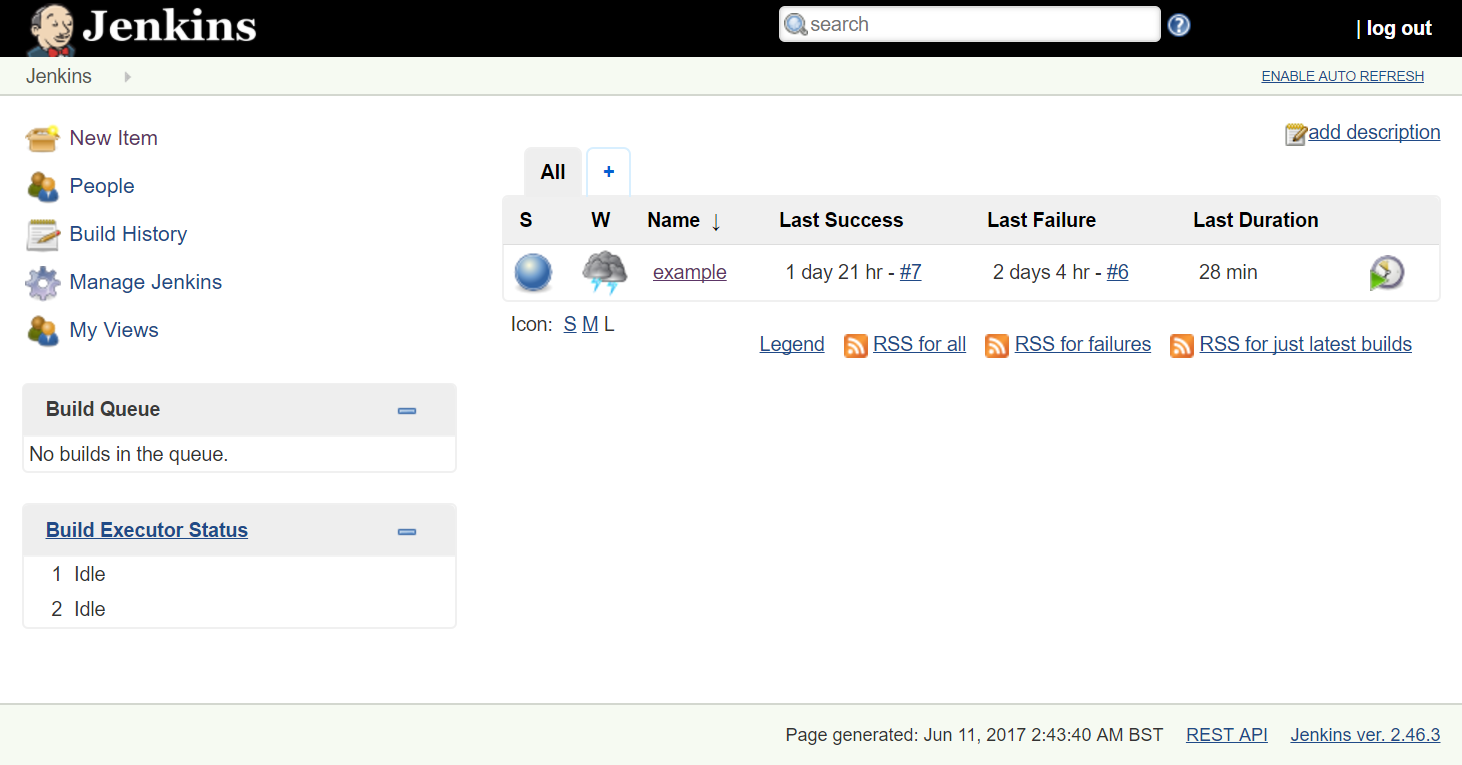
\includegraphics[width=0.9\textwidth]{images/jenkinshome.png}
\end{figure}
As show in Figure \ref{fig:jenkins}, Jenkins provides a web GUI where users can configure the system, create automation jobs and monitor the status of jobs. A job is called a "project", and is commonly a continuous integration cycle of building an application from source code and executing tests for the application. The main page of the Jenkins web GUI shows a list of all defined projects, and statistics about the status of the project. A project in Jenkins always terminates with one of two outcomes: success or failure. A project in Jenkins is defined by a set of user defined rules. These rules are usually one of the following categories:
\begin{itemize}
\item Source Code management - Jenkins can be configured to retrieve source code from version control tools including Git and Subversion.
\item Build trigger - by default all jobs can be started manually from the web GUI. It can also be configured to be started by remote api calls, or by user defined triggers such as the end of another Jenkins job, at user defined intervals, or when the source code is detected to have been updated.
\item Build steps - Jenkins can build Apache Maven based projects, and/or execute any user defined shell scripts and Windows batch commands.
\item After build actions - Jenkins can be configured to store build artifacts, store reports, and trigger other builds.
\end{itemize}
The generality of build steps that can involve any user defined shell script makes it possible to use Jenkins for automating any task that is not limited to building and testing applications.\\
Jenkins projects are also dynamic, and a set of parameters can be passed to the project when it is started. Users can define names and types of parameters, and the values are to be set whenever the project is triggered. The parameters will be available as environment variables throughout the project cycle. The types of parameters are extensible, with support the following types built-in: \cite{pbuild}
\begin{itemize}
\item Boolean
\item Choice - Categorical options
\item File - file to be uploaded to the workspace
\item String / Multi-line String / Password - various text values
\item Run - URL of a specific run of another Jenkins project
\end{itemize}


\subsubsection{Jenkins Plugins}
Jenkins is open source and provides extensibility through plugins. The plugins provide extra functions, powerful ways to define projects, and integrations with many testing and deployment technologies.
Various development environments are supported through plugins, including: \cite{jenplug}
\begin{itemize}
\item Apache Ant projects
\item Gradle projects
\item .Net projects - MSBuild and MSTest
\item Java projects - JUnit and built-in support for Maven
\item Android - Android emulator
\item iOS - Xcode
\end{itemize}
Developers working with these environments have an established framework to help set up their Jenkins automation routine of building and testing. Jenkins also allows manual configuration to build and test applications developed in other environments and languages, through the ability to execute any user defined shell script. This process requires more customisation and knowledge from the developer to understand build and testing behaviour.

\newpage
\subsection{Eclipse IDE Plugins}
\subsubsection{Eclipse IDE}
Eclipse is a commonly used Integrated Development Environment for Java developers, along with a significant userbase among C/C++ and PHP developers. \cite{eclipseide} It is the developement environment that the DICE project has targeted, and built the DICE IDE upon. \cite{dicetools}\\
\begin{figure}[h]
\centering
\caption{Eclipse IDE user interface. \cite{eclipsescreenshot}}
\label{fig:eclipse}
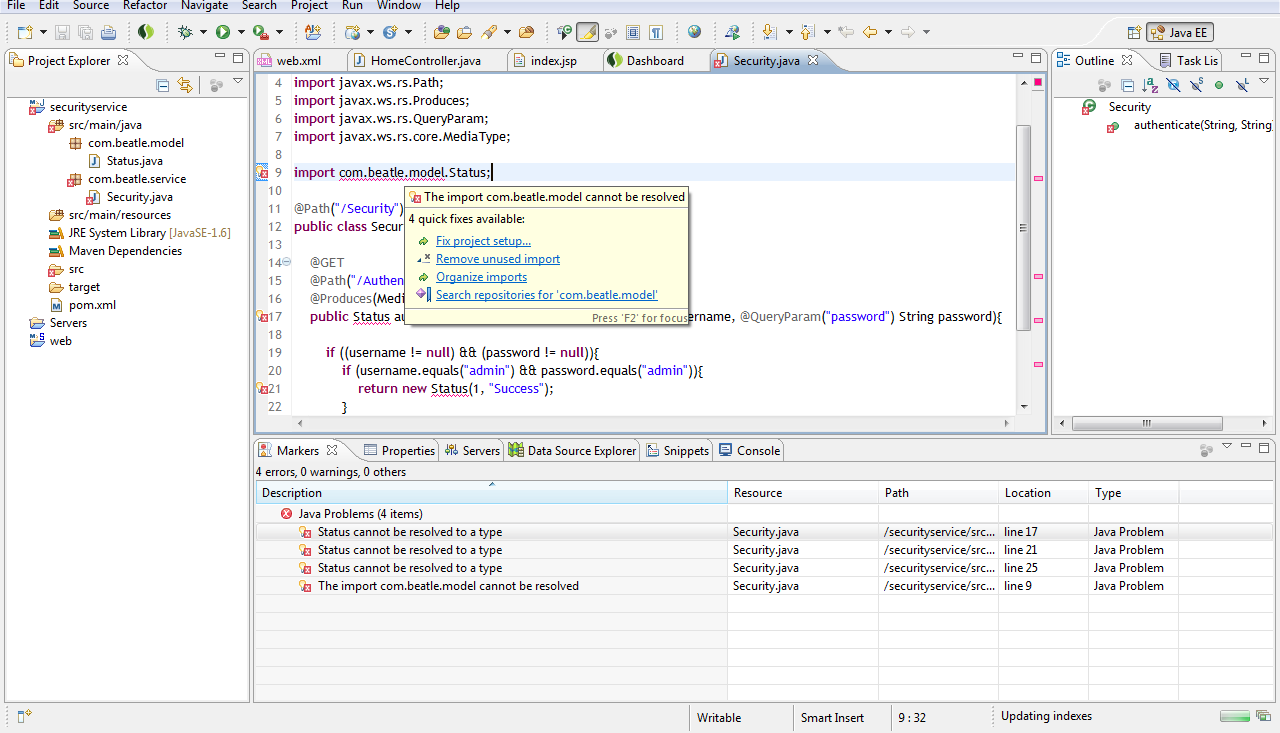
\includegraphics[width=0.9\textwidth]{images/eclipse.png}
\end{figure}
The architecture of Eclipse IDE is based on the principles of modular systems and services, for which the OSGi core framework has set a specification \cite{osgi}. Equinox is an implementation of the framework, and forms the basis of the Eclipse IDE's core runtime system kernel. Eclipse has a concept of a workspace, and all functionality is provided by plugins on top of Equinox, as modular components called bundles. According to the OSGi architecture, bundles are tightly coupled, dynamically loadable collections of classes, jars, and configuration files that explicitly declare any of their external dependencies. This allows all functionlity and plugins in Eclipse to integrate into the system in the same way.\\
With this architecture, the Eclipse IDE allows extensive customisation and easy extension support developement in different languages, and add fucntions such as configuration management and version control. Development environments are provided for the following languages: \cite{eclipsepkgs}
\begin{itemize}
\item Java - Eclipse Java development tools (JDT), with advanced refactoring techniques and code analysis
\item C and C++ - Eclipse C development tools (CDT)
\item PHP - Eclipse PHP development tools (PDT)
\item Android - Eclipse for Android Developers
\item Javascript - Eclipse IDE for JavaScript and Web Developers
\end{itemize}
Development for the following programming languages are supported via plugins: \cite{eclipsemarket}
\begin{multicols}{3}
\begin{itemize}
\item Ada
\item ABAP
\item Clojure
\item COBOL
\item D
\item Erlang
\item Fortran
\item Groovy
\item Haskell
\item Julia
\item Lasso
\item Lua
\item NATURAL
\item Perl
\item Prolog
\item Python
\item R
\item Ruby, Ruby on Rails
\item Rust
\item Scala
\item Scheme
\item TeXlipse - development of LaTeX documents
\end{itemize}
\end{multicols}
Other plugins in eclipse provide integrations and additional functionality: \cite{eclipsemarket}
\begin{itemize}
\item EGit - integration of Git version control system
\item Subversive - integrationi of Subversion (SVN) version control system
\item Buildship Gradle Integration
\item m2e - Maven integration
\item Checkstyle - source code analyzer Checkstyle.
\item Eclipse Memory Analyzer - Java heap analyzer
\end{itemize}
The Eclipse UI is built upon the Standard Widget Toolkit (SWT, a Java toolkit that contains graphical control elements. It also uses JFace as the intermediate graphical user interface layer to simplify application construction.

\subsubsection{Eclipse and Jenkins}

Following the DevOps principles of testing in production environment, automation and remote deployment of application, we investigate the current state of integration in the development environment (Eclipse IDE) and the build automation tool (Jenkins). The current integration is provided via the "Hudson/Jenkins Mylyn Builds Connector" under the Mylyn task and application lifecycle management (ALM) framework for Eclipse. \cite{mylyn}\\
The plugin describes itself as a "View to review, start builds in CI server", and lists the following features:
\begin{itemize}
\item connect to many Hudson/Jenkins instances, filtered list of jobs
\item view build logs in Eclipse, error stacks are clickable to open classes
\item view JUnit results, and rerun them locally
\end{itemize}
\begin{figure}[h]
\centering
\caption{Hudson/Jenkins Mylyn Builds Connector user interface. \cite{mylyn}}
\label{fig:mylyn}
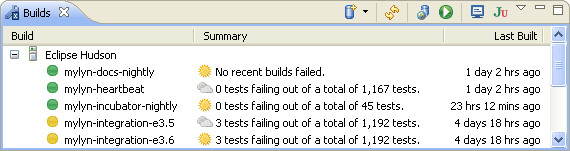
\includegraphics[width=0.9\textwidth]{images/mylyn.png}
\end{figure}
Figure \ref{fig:mylyn} shows the user interface of the Hudson/Jenkins Mylyn Builds Connector. It mimics the summary view of the main Jenkins web GUI landing page shown in Figure \ref{fig:jenkins}. This demonstrates the ability to log in to a secure Jenkins server with the provided credentials, and retrieve the status of projects. The ability to start a build has been investigated, and it was found that the plugin is only capable of starting basic builds that did not require any parameters. Parameterized builds were not supported by the plugin, and it also did not provide the functionality to create and define new project builds.

\subsubsection{Eclipse Plugin Development}
As described in the sections above, all functionality in Eclipse are provided via plugins. The Eclipse IDE can be extensively extended with any functionality by developing plugins on top of the platform. This is an implementation of the OSGi framework and its principles: to have a modular system; where eclipse plugins are implementations of OSGi bundles.\\
Even the Eclipse IDE itself can be seen as an extension and implementation of the Eclipse RCP, with the function to aid software development. Although released as a whole package, these software development functionalities of the IDE are actually sets of plugins to the system, such as the Java Development Tools and C development tools. When these plugins are uninstalled, Eclipse IDE is still capable of launching as an application without any development support functionality.\\
Eclipse for RCP and RAP Developers is the package that includes a set of plugins to form the Eclipse plugin development environment (PDE). These tools provide the following functionalities: \cite{vogella}
\begin{itemize}
\item project creation wizard - configure and build plugins from style templates
\item dependency management - Manifest
\item launch, test and debug - launch a new eclipse instance with plugin built and installed for testing
\end{itemize}
When a plugin project is started from the project creation wizard, the project directory structure is configured automatically, along with plugin dependencies, metadata and the manifest file. The developer manually create a custom plugin from scratch, or select from the following types of plugin templates to suit the style and purpose of their plugin:
\begin{itemize}
\item Plugin with a multi-page editor
\item Plugin with a popup menu
\item Plugin with a property page
\item Plugin with a view
\item Plugin with an Eclipse 4 handler
\item Plugin with an Eclipse 4 view
\item Plugin with an editor
\item Plugin with an incremental project build
\item Plugin with sample help content
\end{itemize}
Each of the templates provide the UI's top level display style as a blank canvas with some sample control buttons for demonstration purpose. Developers can add their own controls to the top level display according to the SWT toolkit. In the SWT toolkit, all UI elements such as the display canvas, text, and buttons, are controls that follow a tree type hierarchy from the top level display provided by the template.

\subsubsection{SWT: The Standard Widget Toolkit}
The Standard Widget Toolkit (SWT) provides Java developers with widgets that tightly integrate with the underlying native OS GUI platform, with an API that is portable across various platforms. The API across platforms is common, but implemented with platform native widgets when they are available. Therefore SWT reflects the native look and feel of the underlying OS GUI \cite{swt}, and any changes to its style. The native OS's GUI libraries is accessed via Java Native Interface in order to display GUI elements. In this sense, SWT is similar to programs written using APIs specific to each operating system.\\
As SWT uses native objects that are not tracked by the Java JVM, the JVM's garbage collection mechanism cannot track the usage of these objects, and cannot automate the garbage collection of SWT widgets. Therefore SWT is different from any other Java toolkit in that it requires manual deallocation of objects created. The deallocation is invoked by a call to the dispose method implemented by all SWT widgets. \cite{swtwidget} Each SWT widget handles the disposal of the native OS objects or delegates disposal to lower level widgets by invoking their dispose method.\\

The core architecture of SWT is formed by widgets, layouts and events. As a comparison to the MVC model, widgets are graphical objects that also contain data, layouts are specifications of GUI style, and events hold the logic and actions in response to user interaction.\\
The main execution entry point of the UI is the Display. It manages communication with the OS's GUI system, and coordinates the event loop. \cite{swtwidget}\\
The Display will contain top level Shells as its children. Shells are the visually represented as "windows" by the underlying OS. They can be moved, resized, minimized and maximized, and may contain shells within shells, for example pop-ups and dialogue boxes that are entirely "contained" by another window.\\
This concept of "containing" gives rise to the widget's hierarchical structure. The shell / application window is at the top of the hierarchy, as the root of a tree. The shell will have other widgets as children, and those widgets may in turn contain more widgets further down the tree levels. As a rule, all widgets that are not top level shells must have a parent. Top level shells do not have a parent, but they are created in association with a particular Display. All other widgets are created as descendants (direct or indirect) of top level shells.\\
The Control class is a general abstract class of widgets that can be placed at any level of the hierarchical tree, while the Composite class are widgets that can contain other widgets, i.e. can have children. \cite{swtcontrol}\\
\begin{figure}
\centering
\caption{SWT Widgets \cite{swtwidgets}}
\label{fig:swt}
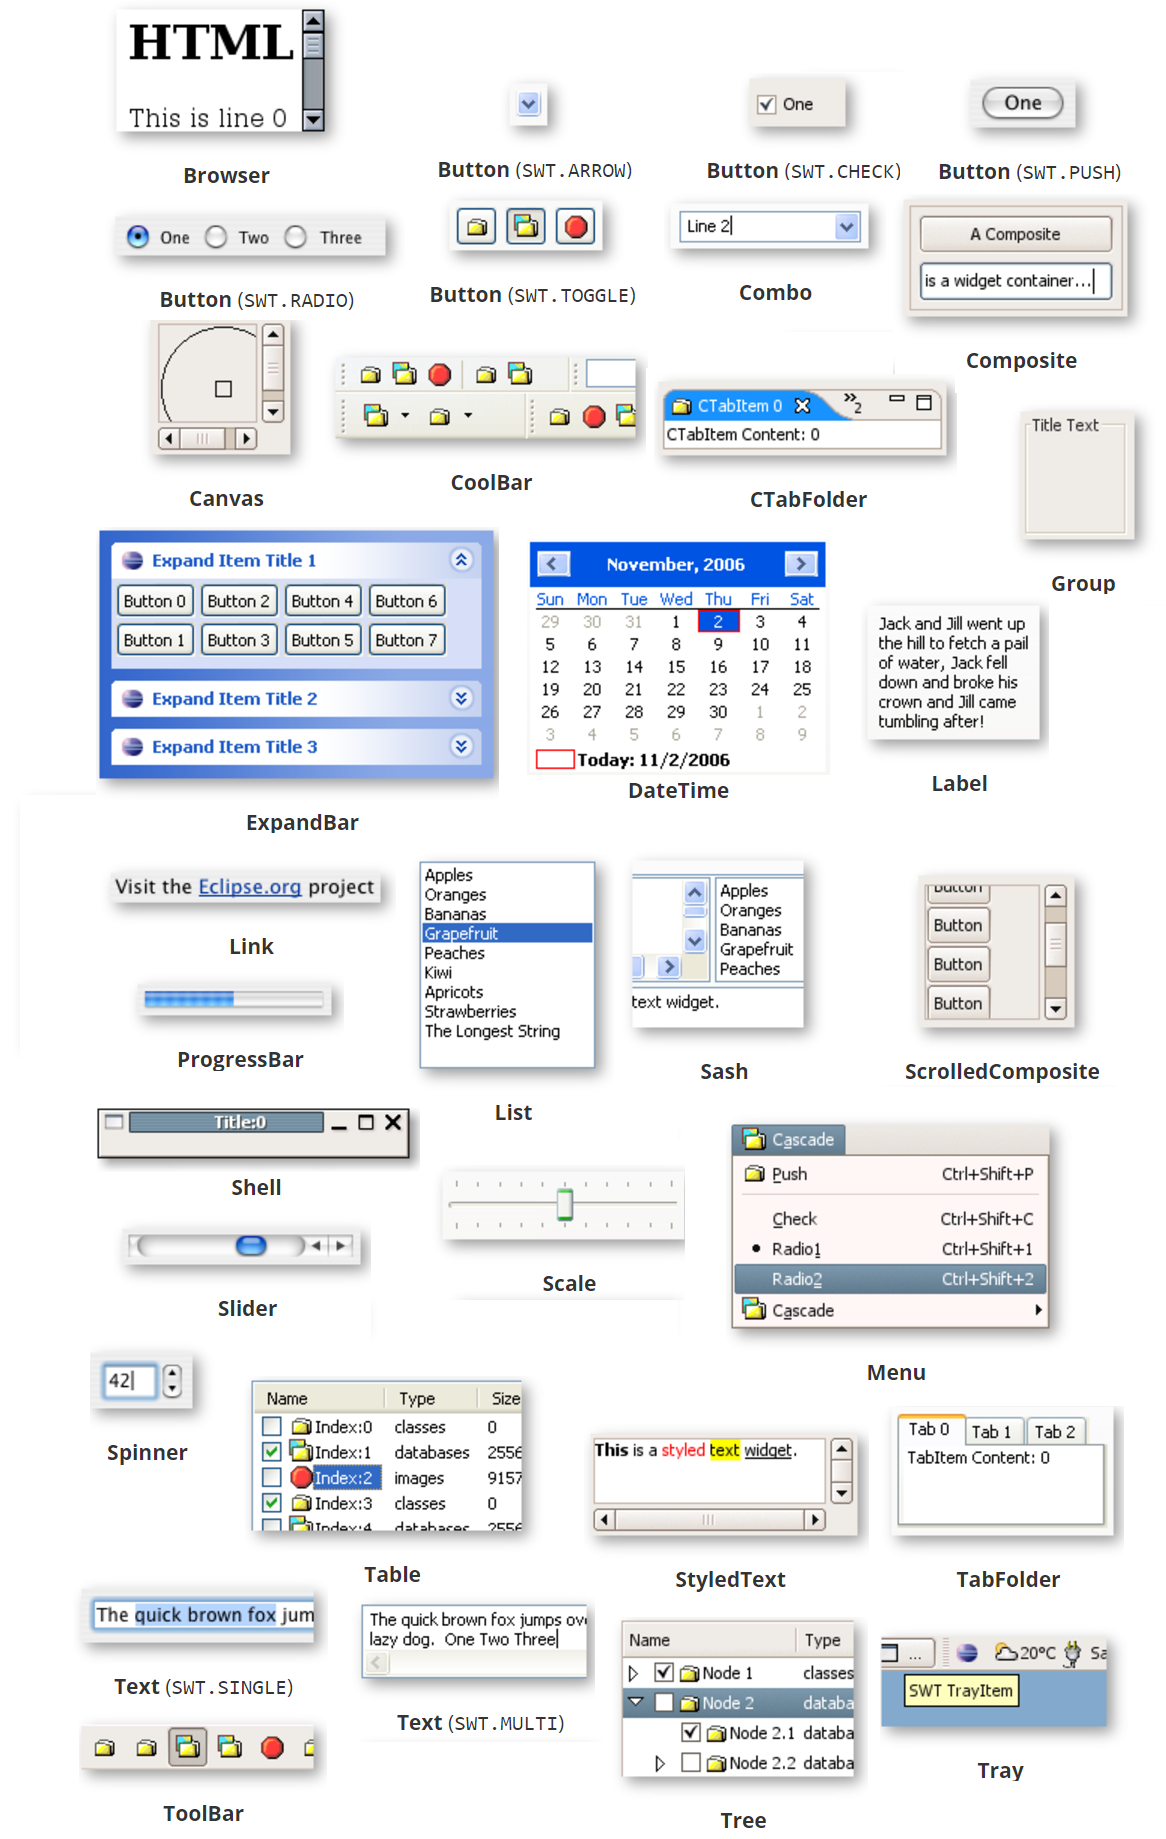
\includegraphics[width=1\textwidth]{images/swt.png}
\end{figure}
Figure \ref{fig:swt} shows screen shots of SWT widgets, while the detailed description can be found in the appendix.\\

The appearance and positioning of widgets can be modified by style bits and layout. \cite{swtlayout} Style bits set in the constructor of widgets determine properties such as whether widget has border outline, and whether the widget has scroll bars. A widget may have many style properties, represented by the bitwise OR of all style bits. When the selected style is not available on a platform, it is ignored.\\

The event and listener pattern is used to control logic and respond to user interaction in SWT. Messages are passed to widgets from the application's message loop, containing information about events from the queue. Widgets then notify their listeners for the specific event, and the listener contains logic to respond to the event. Listener interfaces are defined for different types of listeners, to specific what trigger events they should react to. For example, a "open" button's selection listener will listen to selection events, i.e. when the button is pressed, and execute the related code for the "open" action as defined by the developer.\\
Events are divided into two categories, where low level events describe specific user interactions, and high level events are logical operations or controls that may be formed of multiple low level events. \cite{swtevent} The details of SWT events can be found in the appendix.